\documentclass[dvipsnames]{beamer}
\usepackage{graphicx}
\usepackage{listings}
\usepackage{adjustbox}
\usepackage{xcolor}

\definecolor{PastelGreen}{HTML}{1A7A67}
\definecolor{PastelBlue}{HTML}{2C3E50}
\definecolor{PastelWhite}{HTML}{FAF8F6}
\definecolor{PastelLilac}{HTML}{A391C1}
\definecolor{PastelRed}{HTML}{FAA0A0}

\definecolor{TrenordBlue}{HTML}{006297}
\definecolor{TrenordLightGreen}{HTML}{b6dd79}
\definecolor{TrenordDarkGreen}{HTML}{79be20}
\definecolor{TrenordFalseGreen}{HTML}{d6e965}

\definecolor{FERRed}{HTML}{d9585d}
\definecolor{FERDarkGreen}{HTML}{369389}
\definecolor{FERLightGreen}{HTML}{44a25a}

\definecolor{ATMRed}{HTML}{ef1a2f}
\definecolor{ATMGreen}{HTML}{5d982e}
\definecolor{ATMYellow}{HTML}{fdb90b}
\definecolor{ATMBlue}{HTML}{14386a}
\definecolor{ATMLilac}{HTML}{9a8fc5}

\definecolor{XMPRGreen}{HTML}{00685e}
\definecolor{XMPRBlue}{HTML}{003da5}
\definecolor{XMPRGray}{HTML}{474b4e}

\usetheme{Madrid}

%% FER
% \setbeamercolor{palette primary}{bg=FERDarkGreen,fg=white}
% \setbeamercolor{author in head/foot}{bg=FERLightGreen,fg=black}
% \setbeamercolor{title in head/foot}{bg=FERRed,fg=black}
% \setbeamercolor{date in head/foot}{bg=FERDarkGreen,fg=black}

%% TRENORD
\setbeamercolor{palette primary}{bg=TrenordBlue,fg=white}
\setbeamercolor{author in head/foot}{bg=TrenordLightGreen,fg=black}
\setbeamercolor{title in head/foot}{bg=TrenordDarkGreen,fg=black}
\setbeamercolor{date in head/foot}{bg=TrenordFalseGreen,fg=black}

%% ATM
% \setbeamercolor{palette primary}{bg=ATMGreen,fg=white}
% \setbeamercolor{author in head/foot}{bg=ATMRed,fg=black}
% \setbeamercolor{title in head/foot}{bg=ATMYellow,fg=black}
% \setbeamercolor{date in head/foot}{bg=ATMLilac,fg=black}

%% XMPR
% \setbeamercolor{palette primary}{bg=XMPRGreen,fg=white}
% \setbeamercolor{author in head/foot}{bg=XMPRBlue,fg=white}
% \setbeamercolor{title in head/foot}{bg=XMPRBlue,fg=white}
% \setbeamercolor{date in head/foot}{bg=XMPRBlue,fg=white}
% \setbeamercolor{structure}{fg=XMPRGray}

\usecolortheme[named=PastelBlue]{structure}

\date[03 June 2025]{}

\title[AOGA]{Efficient transit network design and frequencies setting multi-objective optimization by Alternating Objective Genetic Algorithm}
\subtitle{Renato~Oliveira~Arbex, Claudio~Barbieri~da~Cunha}
\author[Francesco~Refolli]{}
\logo{
\includegraphics[height=2.5cm]{logo_unimib.pdf}}

\begin{document}

\frame{\titlepage}

\setbeamertemplate{logo}{}

\begin{frame}
  \frametitle{Problem statement / 1}

  \begin{definition}
    The \textit{Transit Network Design and Frequency Setting Problem} (\textbf{TNDFSP})
    \begin{itemize}
      \item requires to compute a set of Service Lines (\textit{routes} + \textit{trip frequencies})
      \item given the Infrastructure Network and its associated Demand Matrix.
    \end{itemize}
  \end{definition}

  \begin{columns}
    \begin{column}{0.5\textwidth}
      \begin{figure}
        \centering
        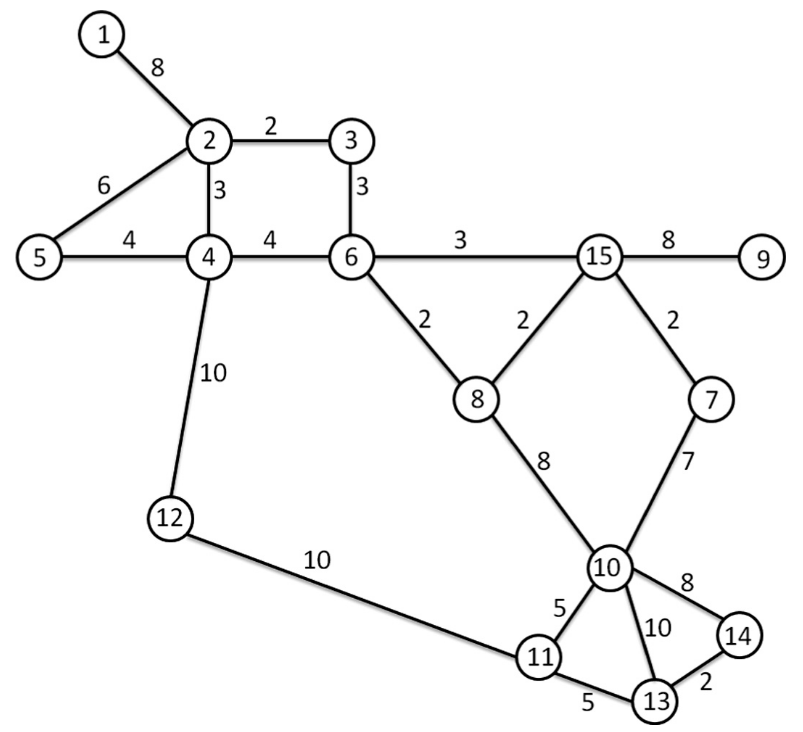
\includegraphics[width=0.7\textwidth]{figures/example-input-network.png}
        \caption{Example of INPUT Network}
      \end{figure}
    \end{column}
    \begin{column}{0.5\textwidth}
      \begin{figure}
        \centering
        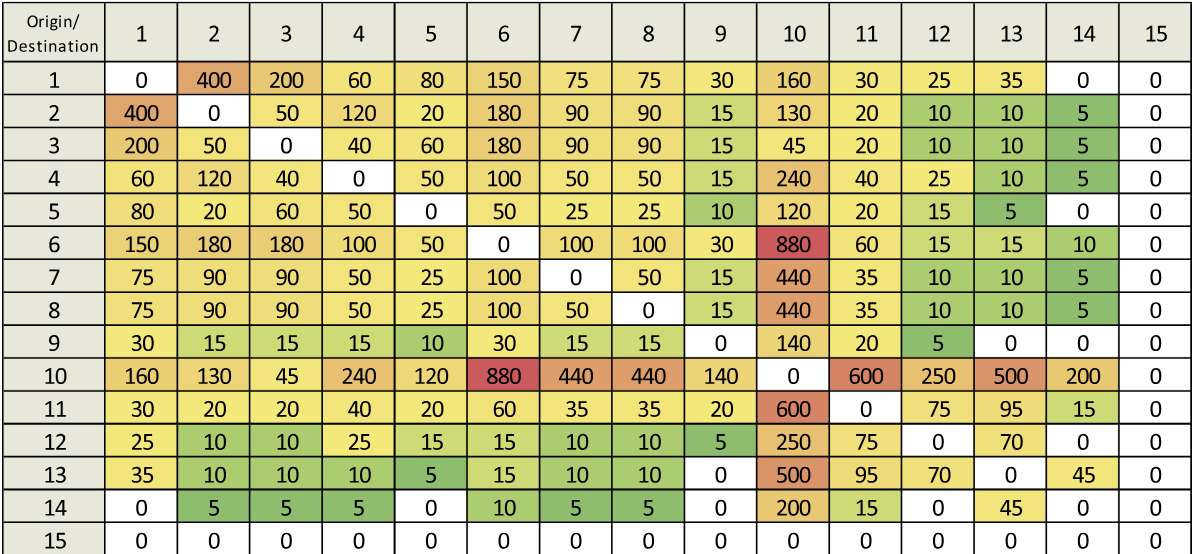
\includegraphics[width=1.00\textwidth]{figures/example-input-demand.png}
        \caption{Example of INPUT Demand}
      \end{figure}
    \end{column}
  \end{columns}
\end{frame}

\begin{frame}
  \frametitle{Problem statement / 2}

  \begin{definition}
    The \textit{Transit Network Design and Frequency Setting Problem} (\textbf{TNDFSP})
    \begin{itemize}
      \item requires to compute a set of Service Lines (\textit{routes} + \textit{trip frequencies})
      \item given the Infrastructure Network and its associated Demand Matrix.
    \end{itemize}
  \end{definition}

  \begin{figure}
    \centering
    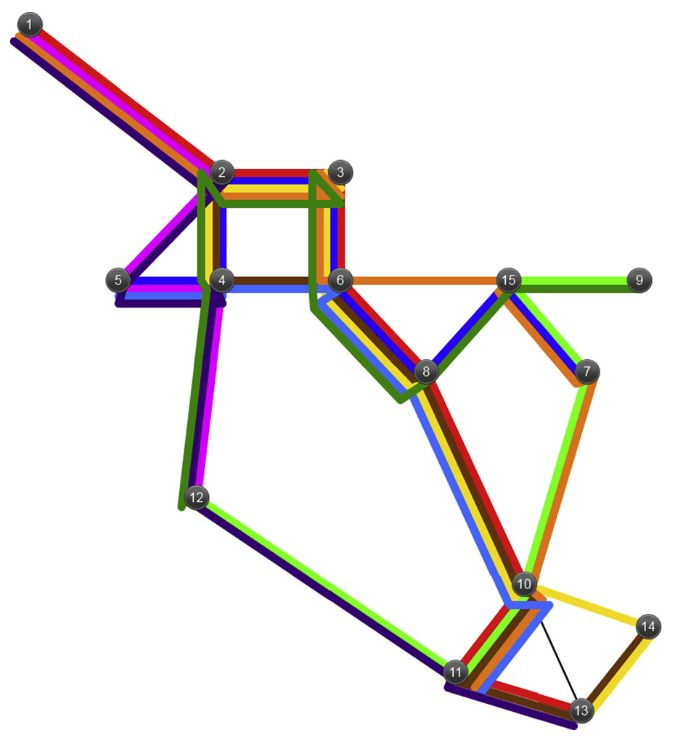
\includegraphics[width=0.3\textwidth]{figures/example-output-lines.png}
    \caption{Example of OUTPUT Lines}
  \end{figure}
\end{frame}

\begin{frame}
  \frametitle{Problem statement / 3}
 
  \begin{block}{Objective Functions}
    \begin{equation}
      \label{eq:F1-F2}
      \begin{array}{l}
        min \; F_1 = C_{wt} \times TWT + TIVIT + \Sigma _ {\alpha = 1} ^ {2} C_{\alpha t} \times T\alpha T + C_{ud} \times UD \\
        min \; F_2 = \Sigma _ {s \in S} VN_{s}
      \end{array}
    \end{equation}
  \end{block}
 
  \begin{itemize}
    \item $TWT$ total waiting time for all passengers
    \item $C_{wt}$ waiting time weight
    \item $TIVTT$ total in-vehicle travel time for all passengers
    \item $T\alpha T$ total number of \textit{$\alpha$-th} transfers required by all passengers
    \item $C_{\alpha t}$ \textit{$\alpha$-th} transfer penalty
    \item $UD$ unsatisfied demand
    \item $C_{ud}$ penalty for unsatisfied demand
    \item $VC_{s}$ fleet size of one service line
  \end{itemize}
\end{frame}

\begin{frame}
  \frametitle{Problem statement / 4}
 
  \begin{alertblock}{Rules}
    \begin{itemize}
      \item A solution is a set of unique Service Lines forming a connected component covering the entire input network.
      \item A route is a path (of min length = $3$) from a node \textit{A} to a node \textit{B} without repetitions of nodes.
      \item Each bus has 40 seats and cannot hold more than 50 passengers.
    \end{itemize}
  \end{alertblock}
\end{frame}

\begin{frame}
  \frametitle{A Genetic Algorithm for TNDFSP}
  \begin{figure}
    \centering
    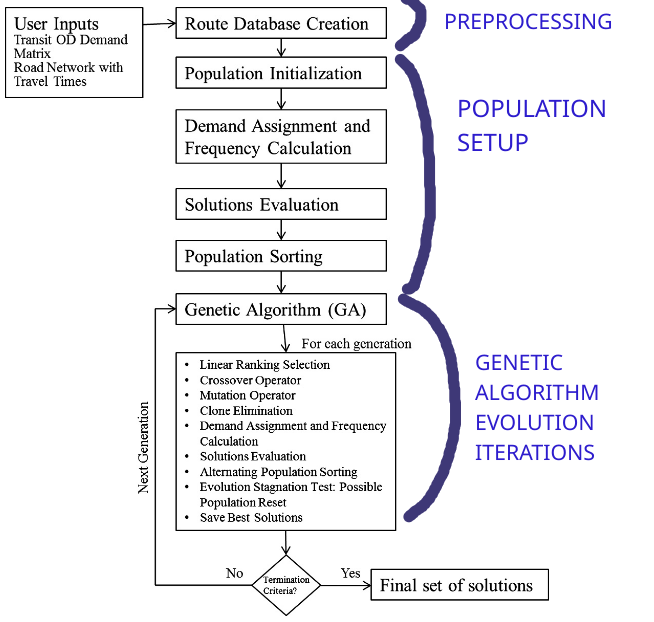
\includegraphics[width=0.7\textwidth]{figures/flowchart-annotated.png}
  \end{figure}
\end{frame}

\begin{frame}
  \frametitle{Route Database Creation / 1}

  \begin{block}{Definition}
    \begin{itemize}
      \item The Route DB is a collection of paths.
      \item Each path is contained exaclty once and has an associated ID.
      \item The Route DB is indexed so that it is possible to retrieve in $O(1)$ all the paths starting with node $v$, ending with node $w$ or containing the edge $(v, w)$
    \end{itemize}
  \end{block}
\end{frame}

\begin{frame}
  \frametitle{Route Database Creation / 2}
  \begin{block}{Route DB Construction}
    \begin{itemize}
      \item For each pair of nodes $(v, w) \in V \times V$ such that $OD[v, w] \neq 0$, add the \textit{k-shortest-paths} from $v$ to $w$.
      \item $k$ is not fixed but is expressed as \textit{detour ratio} $R \in (0,1)$.
      \item Calling $C_p$ the cost of the path $p$ and $C_{o}$ the minimal cost of a shortest path, it selects all paths $p$ such that $\frac {C_p - C_o} {C_o} \leq R$.
      \item The \textit{k-shortest-paths} for a pair $v, w$ are obtained using the \textbf{Yen} Algorithm, which in turn uses the \textbf{Dijkstra} algorithm on increasingly modified versions of the adjacency matrix of the graph.
    \end{itemize}
  \end{block}
\end{frame}

\begin{frame}
  \frametitle{Route Database Creation / 3}
  \begin{alertblock}{Construction Time Complexity}
    \begin{itemize}
      \item The Dijkstra Algorithm is $O(|E|+|V|log|V|)$
      \item The Yen Algorithm calls Dijkstra $k|V|$ times
      \item Assuming verifying path membership is $O(1)$.
      \item Assuming adding a path to the DB is $O(1)$.
      \item Constructing Route DB is $O(k|V|^3(|E|+|V|log|V|))$
    \end{itemize}
  \end{alertblock}

  \begin{alertblock}{Construction Space Complexity}
    \begin{itemize}
      \item The Dijkstra Algorithm is $\Theta(|V|)$
      \item The Yen Algorithm produces $k$ paths with $\Theta(k|V|)$ space
      \item Constructing Route DB is $O(k|V|^3)$
    \end{itemize}
  \end{alertblock}
\end{frame}

\begin{frame}
  \frametitle{Population Initialization / 1}
  \begin{block}{Individual's Generation}
    \begin{itemize}
      \item An \textit{isolated node} has only $1$ edge connecting it to the network (e.g. nodes 1, 9)
      \item For each \textit{isolated node} $v$, add a random route starting/ending with $v$
      \item Track down which nodes are \textit{served} by the current solution
      \item Until all nodes are served: randomly select a pair of unserved nodes $v, w$ such that $OD[v, w] \leq 0$
      \item Add a random route containing the edge $v, w$
      \item Everytime check if the route is already in the solution (then select another one)
      \item If not all nodes can be served, the individual is discarded and a new one is generated instead
    \end{itemize}
  \end{block}
\end{frame}

\begin{frame}
  \frametitle{Population Initialization / 2}
  \begin{alertblock}{Individual's Feasibility Criteria}
    \begin{itemize}
      \item Each node of the graph must be served and the individual shall form a connected component
      \item Each route shall contain at most one occurence of a node
      \item Each individual shall contain at most one occurrence of each row
    \end{itemize}
  \end{alertblock}

  \begin{exampleblock}{Example of Individual}
    \label{example:individual}
    \begin{columns}
      \begin{column}{0.5\textwidth}
        \begin{itemize}
          \item  \textbf{$R_{1}$} : 1-2-3-6-8-10-11-13
          \item  \textbf{$R_{2}$} : 9-15-7-10-11-12
          \item  \textbf{$R_{3}$} : 7-15-8-6-3-2-4-5
          \item  \textbf{$R_{4}$} : 2-4-6-8-10-11-13-14
          \item  \textbf{$R_{5}$} : 13-14-10-8-6-3-2-4
        \end{itemize}
      \end{column}
      \begin{column}{0.5\textwidth}
        \begin{itemize}
          \item  \textbf{$R_{6}$} : 1-2-5-4-12
          \item  \textbf{$R_{7}$} : 11-10-7-15-6-3-2-1
          \item  \textbf{$R_{8}$} : 5-4-6-8-10-11
          \item  \textbf{$R_{9}$} : 13-11-12-4-5-2-1
          \item \textbf{$R_{10}$} : 9-15-8-6-3-2-4-12
        \end{itemize}
      \end{column}
    \end{columns}
  \end{exampleblock}
\end{frame}

\begin{frame}
  \frametitle{Population Initialization / 3}
  \begin{block}{Individual's Fate}
    \begin{itemize}
      \item Each individual does not contain the routes as values but their ID inside the Route DB
      \item Each crossover operation creates a new entry for the Route DB
      \item A crossover operation could invalidate the individual (\textit{unfeasible})
      \item An individual which is not \textit{feasible} is replaced by a freshly generated one
      \item The individual is assigned with served demand and trip frequencies
      \item The individual is evaluated with respect to User Cost ($F_1$) and Operator Cost ($F_2$)
    \end{itemize}
  \end{block}
\end{frame}

\begin{frame}
  \frametitle{Demand Assignment and Frequency Setting / 1}

  For each pair $v, w$ such that $OD[v, w] \neq 0$, compute the probabilities $P_{j}$ of a user wanting to travel from $v$ to $w$ using the combination of routes $j$.
  Those probabilities can be aggregated on route-level to compute the peak load of the route $Q^{max}_{r}$, and then the frequency $f_r$.
  
  \begin{block}{Probabilities for One/Two Transfer Paths}
    \begin{equation}
      \label{eq:POTTP}
      P_{j} = \frac {e^{-U_j}} {\Sigma _ {i \in Options} e ^ {-U_i}}
    \end{equation}
    \begin{equation}
      \label{eq:UOTTP}
      U_i = T_w \cdot C_{wt} + T_{iv} + \Sigma _ {\alpha = 1} ^ {2} X_{\alpha t} \times C_{\alpha t}
    \end{equation}
  \end{block}
  
  \begin{block}{Probabilities for Direct Paths}
    \begin{equation}
      \label{eq:PDP}
      P_{j} = \frac {f_j} {\Sigma _ {i \in Options} f_j}
    \end{equation}
  \end{block}
\end{frame}

\begin{frame}
  \frametitle{Demand Assignment and Frequency Setting / 2}

  \begin{block}{Frequency-based Bound}
    \begin{equation}
      \label{eq:FR}
      f_r = \frac {Q^{max}_{r}} {LF_r \cdot CAP} \leq f_{r_{max}}
    \end{equation}
  \end{block}

  \begin{itemize}
    \item The frequencies of routes can also be computed by rewriting the equation \textit{(\ref{eq:FR})} into \textit{(\ref{eq:NFR})}.
    \item Thus, all frequencies become parameters (initially set to 1) and incremented iteratively until all coefficients $LF_r$ become $\leq LF_{max}$ \\ (set to 1.25 by authors).
    \item NB: Realistically, frequency shall relate to an integer number of trips during the hour/day period.
  \end{itemize}
  
  \begin{block}{Load-Factor-based Bound}
    \begin{equation}
      \label{eq:NFR}
      LF_r = \frac {Q^{max}_{r}} {CAP \cdot f_r} \leq LF_{max}
    \end{equation}
  \end{block}
\end{frame}

\begin{frame}
  \frametitle{Solutions Evaluation}
    At this point the individual is a set of defined routes + the allocated frequencies (thus the fleet size).
    This is enough to compute the objective functions $F_1$ and $F_2$ on the individual using equations \ref{eq:F1-F2}.

  \begin{exampleblock}{Example of Frequency Setting and Individual Evaluation (see \ref{example:individual})}
    \label{example:fs-ie}
    \begin{columns}
      \hspace{0.25cm}
      \begin{column}{0.3\textwidth}
        \begin{tabular}{|l|c|c|c|c|}
          \hline
          Route & $Q_{max}$ & $f$ & $ht$ & $fl$ \\
          \hline
          \textbf{$R_{1}$} & 519.1 & 10.51 & 5.71 & 12 \\
          \hline
          \textbf{$R_{2}$} & 392.02 & 8.42 & 7.12 & 9 \\
          \hline
          \textbf{$R_{3}$} & 279.65 & 6.78 & 8.85 & 4 \\
          \hline
          \textbf{$R_{4}$} & 441.57 & 9.4 & 6.38 & 9 \\
          \hline
          \textbf{$R_{5}$} & 392.32 & 9.0 & 6.66 & 8 \\
          \hline
          \textbf{$R_{6}$} & 124.08 & 3.72 & 16.12 & 3 \\
          \hline
          \textbf{$R_{7}$} & 710.97 & 13.0 & 4.62 & 13 \\
          \hline
          \textbf{$R_{8}$} & 599.38 & 11.9 & 5.04 & 9 \\
          \hline
          \textbf{$R_{9}$} & 157.14 & 4.27 & 14.05 & 6 \\
          \hline
          \textbf{$R_{10}$} & 142.6 & 4.34 & 13.82 & 4 \\
          \hline
        \end{tabular}
      \end{column}
      \begin{column}{0.1\textwidth}
      \end{column}
      \begin{column}{0.3\textwidth}
        \begin{tabular}{|l|c|}
          \hline
          Param & Value \\
          \hline
          \textbf{$C_{wt}$} & 2.0 \\
          \hline
          \textbf{$C_{1t}$} & 30 \\
          \hline
          \textbf{$C_{2t}$} & 40 \\
          \hline
          \textbf{$f_{max}$} & 13 \\
          \hline
          \textbf{$f_{min}$} & 1 \\
          \hline
          \textbf{$F_{1}$} & 458152 \\
          \hline
          \textbf{$F_{2}$} & 77 \\
          \hline
        \end{tabular}
      \end{column}
    \end{columns}
  \end{exampleblock}
\end{frame}

\begin{frame}
  \frametitle{(Alternating) Population Sorting and Linear Ranking Selection}
  \begin{itemize}
    \item The population is sorted by one of the two objective functions ($F_1$ and $F_2$), alternatively
    \item If in iteration $t$ it was sorted with $F_1$, in iteration $t+1$ it is sorted with $F_2$
    \item The top $k$ individuals out of the sorted population are selected for breeding, the rest is discarded
  \end{itemize}
\end{frame}

\begin{frame}
  \frametitle{Crossover Operator}
  \begin{itemize}
    \item Individuals are selected for crossover with linear ranking
    \item A single point of crossover $k$ is selected randomly
    \item Offsprings are created by exchanging their \textit{k-th} route
    \item Satisfability of offspring is checked and in case of damage, a new crossover point $k'$ is selected
    \item If no more offspring can be generated, a new pair of parents is selected ...
    \item ... until at most 80\% of possible pairs has been processed
  \end{itemize}
\end{frame}

\begin{frame}
  \frametitle{Mutation Operator}
  \begin{itemize}
    \item An individual mutates by replacing one of its routes with another one from the Route DB
    \item The new route is selected so that is serves the same OD Pair that originally generated the route
    \item Again, if the individual cannot be mutated without having an invalid offspring, a new individual is selected for mutation
  \end{itemize}
\end{frame}

\begin{frame}
  \frametitle{Clone Elimination, Stagnation Test and Population Reset}
  \begin{itemize}
    \item If two individuals are (symmetrically) equal, one is discarded and replaced by a newly generated one
    \item (Test) Whenever the lowest fleet and user cost is the same after more than 200 generations ...
    \item (Reset) ... the entire population is renewed using the initial population procedure
    \item The best \textit{k-th} individuals (regardless if they are offsprings or parents) are pushed to the next generation (\textit{elitism})
  \end{itemize}
\end{frame}

\begin{frame}
  \begin{figure}
    \centering
    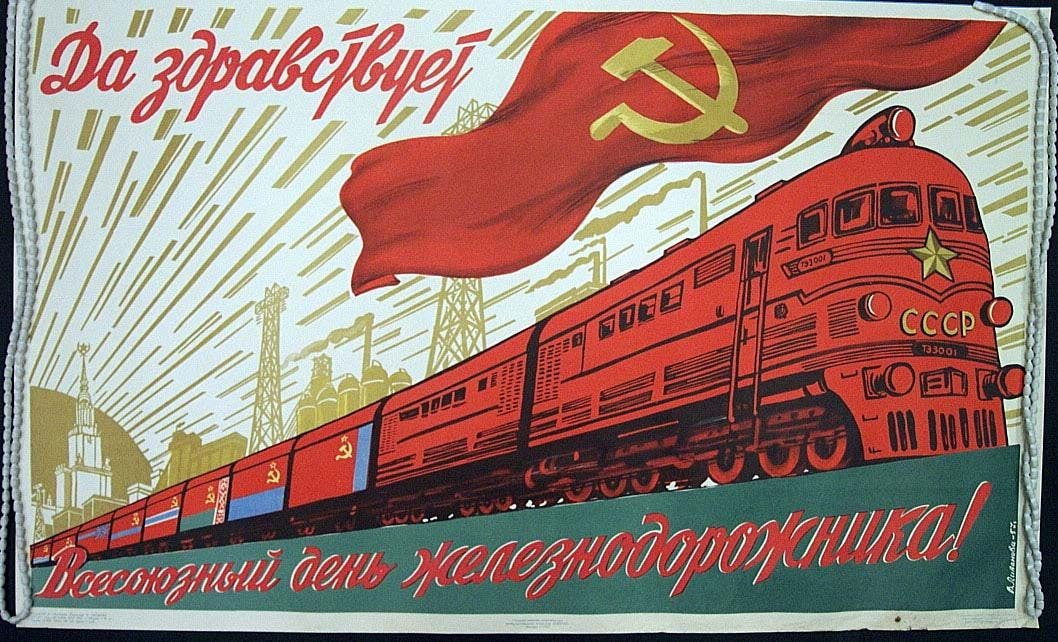
\includegraphics[width=0.9\textwidth]{figures/thankyou.png}
  \end{figure}
\centering
\Huge
Thank You
\end{frame}

\end{document}
